\clearpage
\subsubsection{Igneous}
\begin{table}[h!]
\caption{Categorised GPR profile keywords for igneous environments. Geometry, reflectivity and continuity are shown in separate columns.}
\centering
\small
\begin{tabular}{|p{4.5cm}|p{4.5cm}|p{4.5cm}|}
\hline
\textbf{Geometry} & \textbf{Amplitude / Reflectivity} & \textbf{Continuity} \\
\hline
Concave & Alternating reflectivity & Continuous \\
Concave up structures & Attenuated & Crossing reflectors \\
Fill & High attenuation & Discontinuous \\
Scour & High reflectivity & Horizontal \\
Tangential & Low reflection & Parallel \\
Chaotic & Varied attenuation & Subparallel \\
Complex & Varied reflectivity & Semi-continuous \\
Dipping & & \\
Even & & \\
Hummocky & & \\
Hyperbolic & & \\
Irregular & & \\
Lenticular & & \\
Multidirectional dipping & & \\
Oblique & & \\
Sigmoidal & & \\
Sub-horizontal & & \\
Transparent zones & & \\
Wavy & & \\
Diffraction & & \\
Diffraction hyperbola & & \\
Horizontal layering & & \\
\hline
\end{tabular}
\label{tab:merged_gpr_keywords}
\end{table}

\begin{landscape}
\begin{figure}[h!]
    \centering
    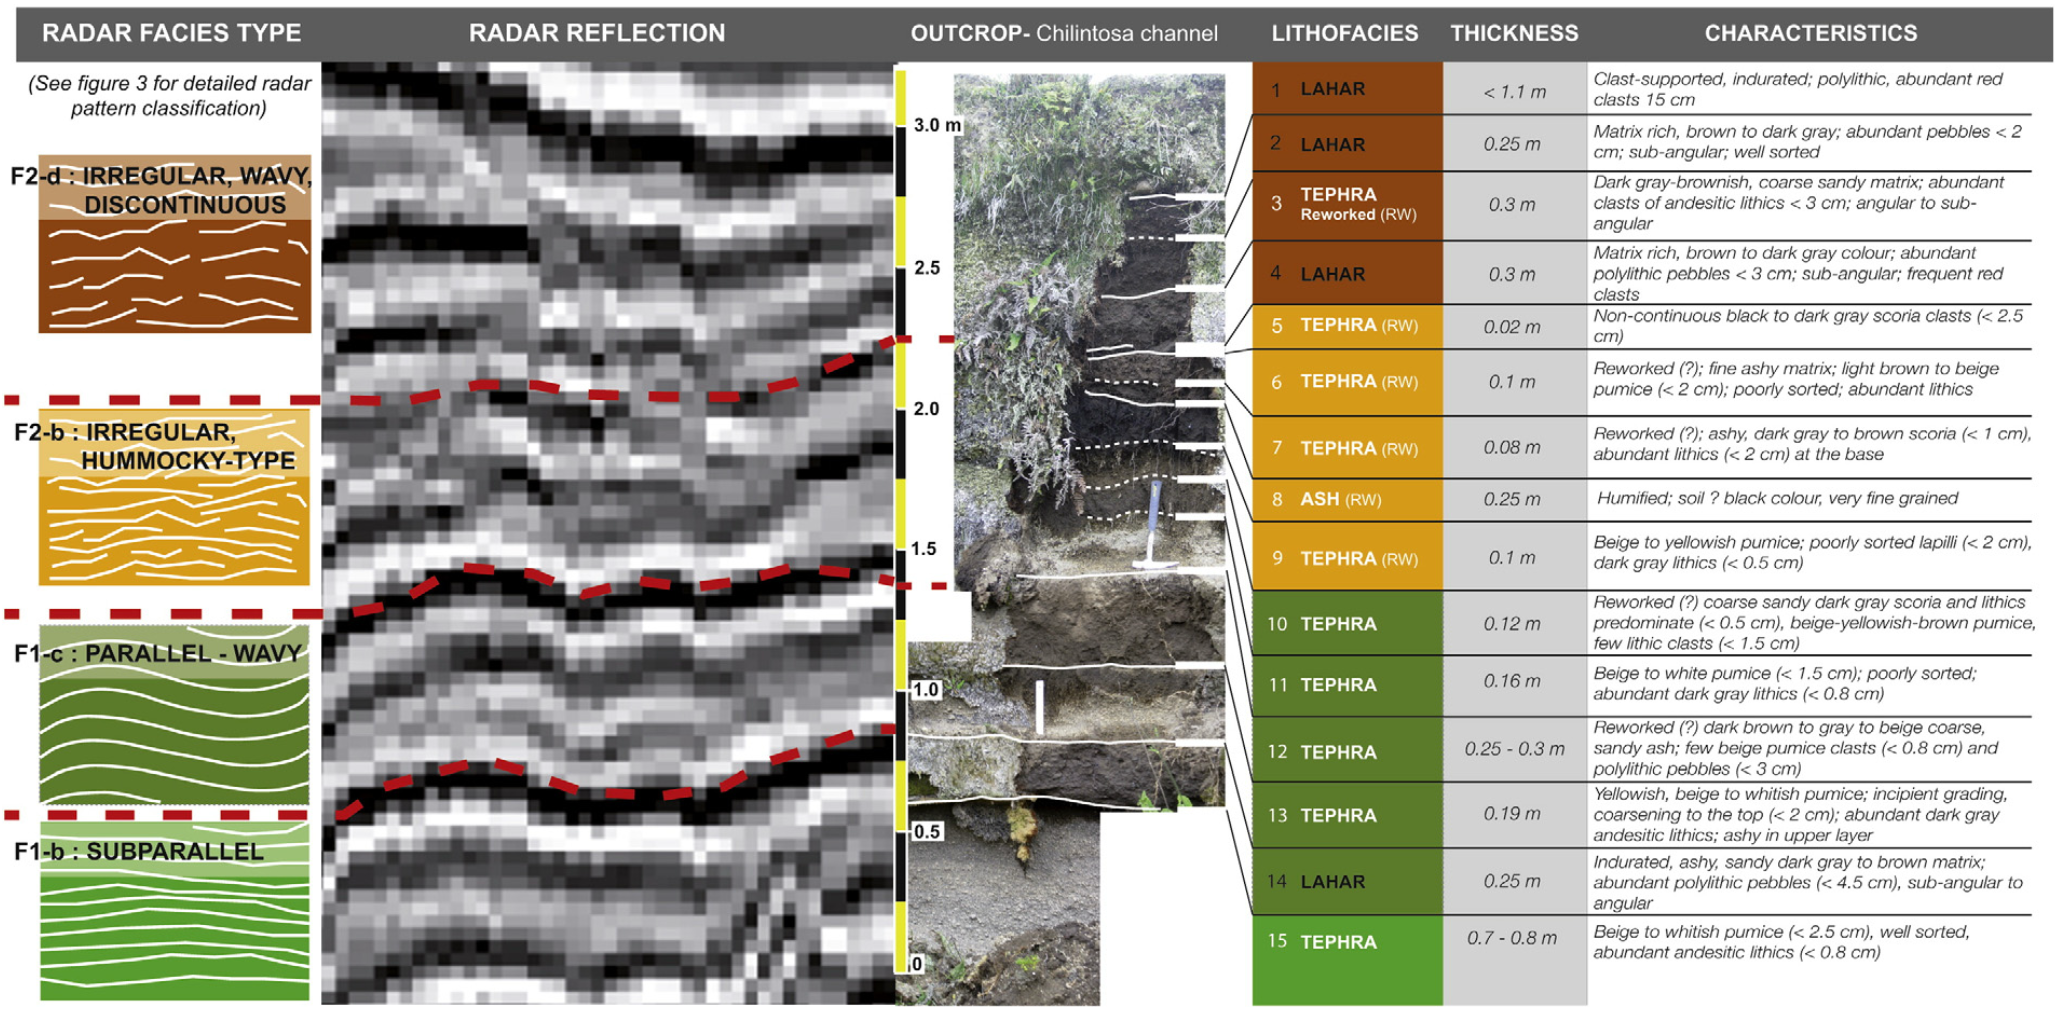
\includegraphics[width=0.9\linewidth]{Figures/0.2GPR/Ettinger2014_lahar_7.png}
    \caption[Lahar-generated fan (1).]{Lahar-generated fan (2). \textbf{Keywords: }Irregular, wavy, discontinuous, hummocky, parallel, subparallel \citep{Ettinger2014}.}
    \label{fig:Ettinger2014-7}
\end{figure}
\end{landscape}

\begin{landscape}
    \begin{figure}[h!]
    \centering
    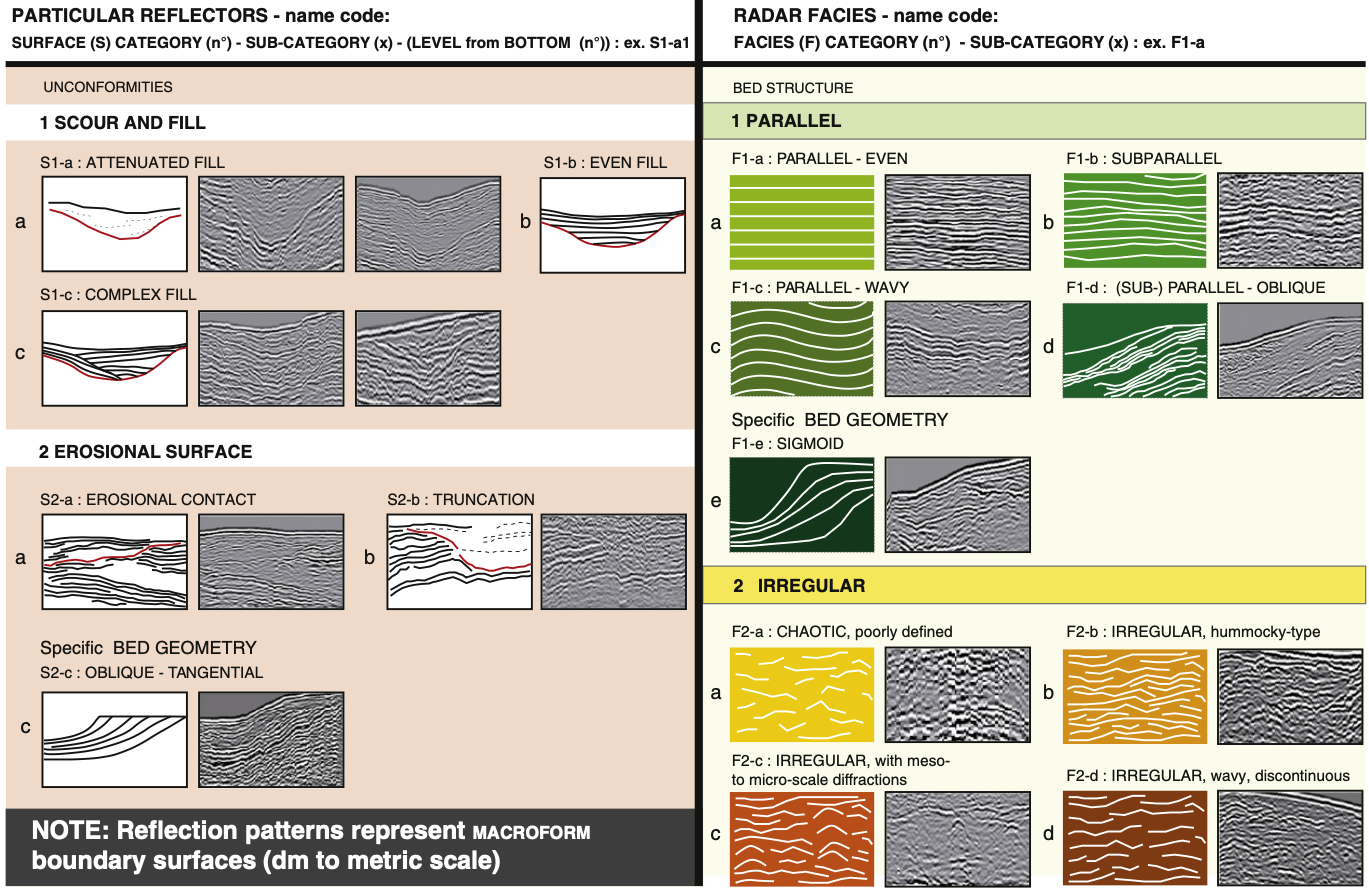
\includegraphics[width=0.9\linewidth]{Figures/0.2GPR/Ettinger2014_lahar_1.png}
    \caption[Lahar-generated fan (2).]{Lahar-generated fan (1). \textbf{Keywords: }Scour, fill, parallel, irregular, even, wavy, sigmoidal, subparallel, oblique, attenuated, complex, truncation, tangential, chaotic, diffraction, hummocky, discontinuous \citep{Ettinger2014}. }
    \label{fig:Ettinger2014-1}
\end{figure}
\end{landscape}
\clearpage

\begin{landscape}
    \begin{figure}[h!]
    \centering
    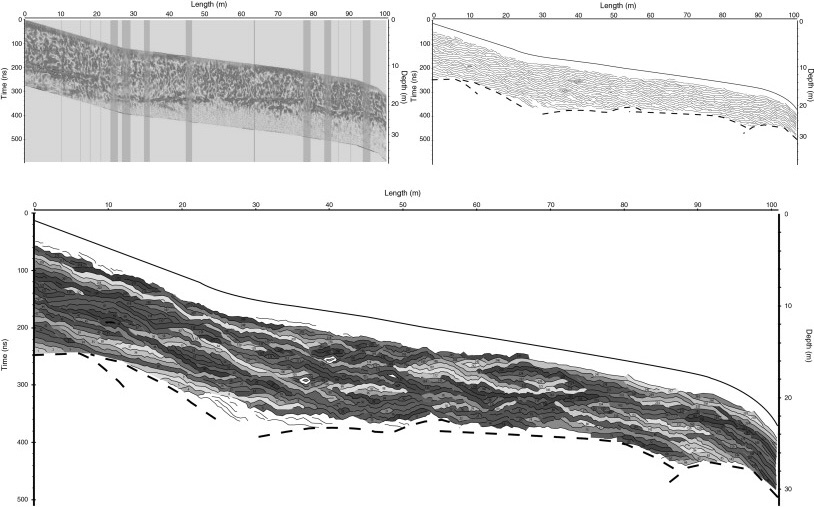
\includegraphics[width=0.9\linewidth]{Figures/0.2GPR/Gomez_2009_pyro.jpg}
    \caption[Pyroclastic flow.]{Pyroclastic flow. \textbf{Keywords: } Varied reflectivity, \citep{Gomez-2009-1}.}
    \label{fig:Gomez2009-1}
\end{figure}
\end{landscape}
\clearpage

\begin{figure}[h!]
    \centering
    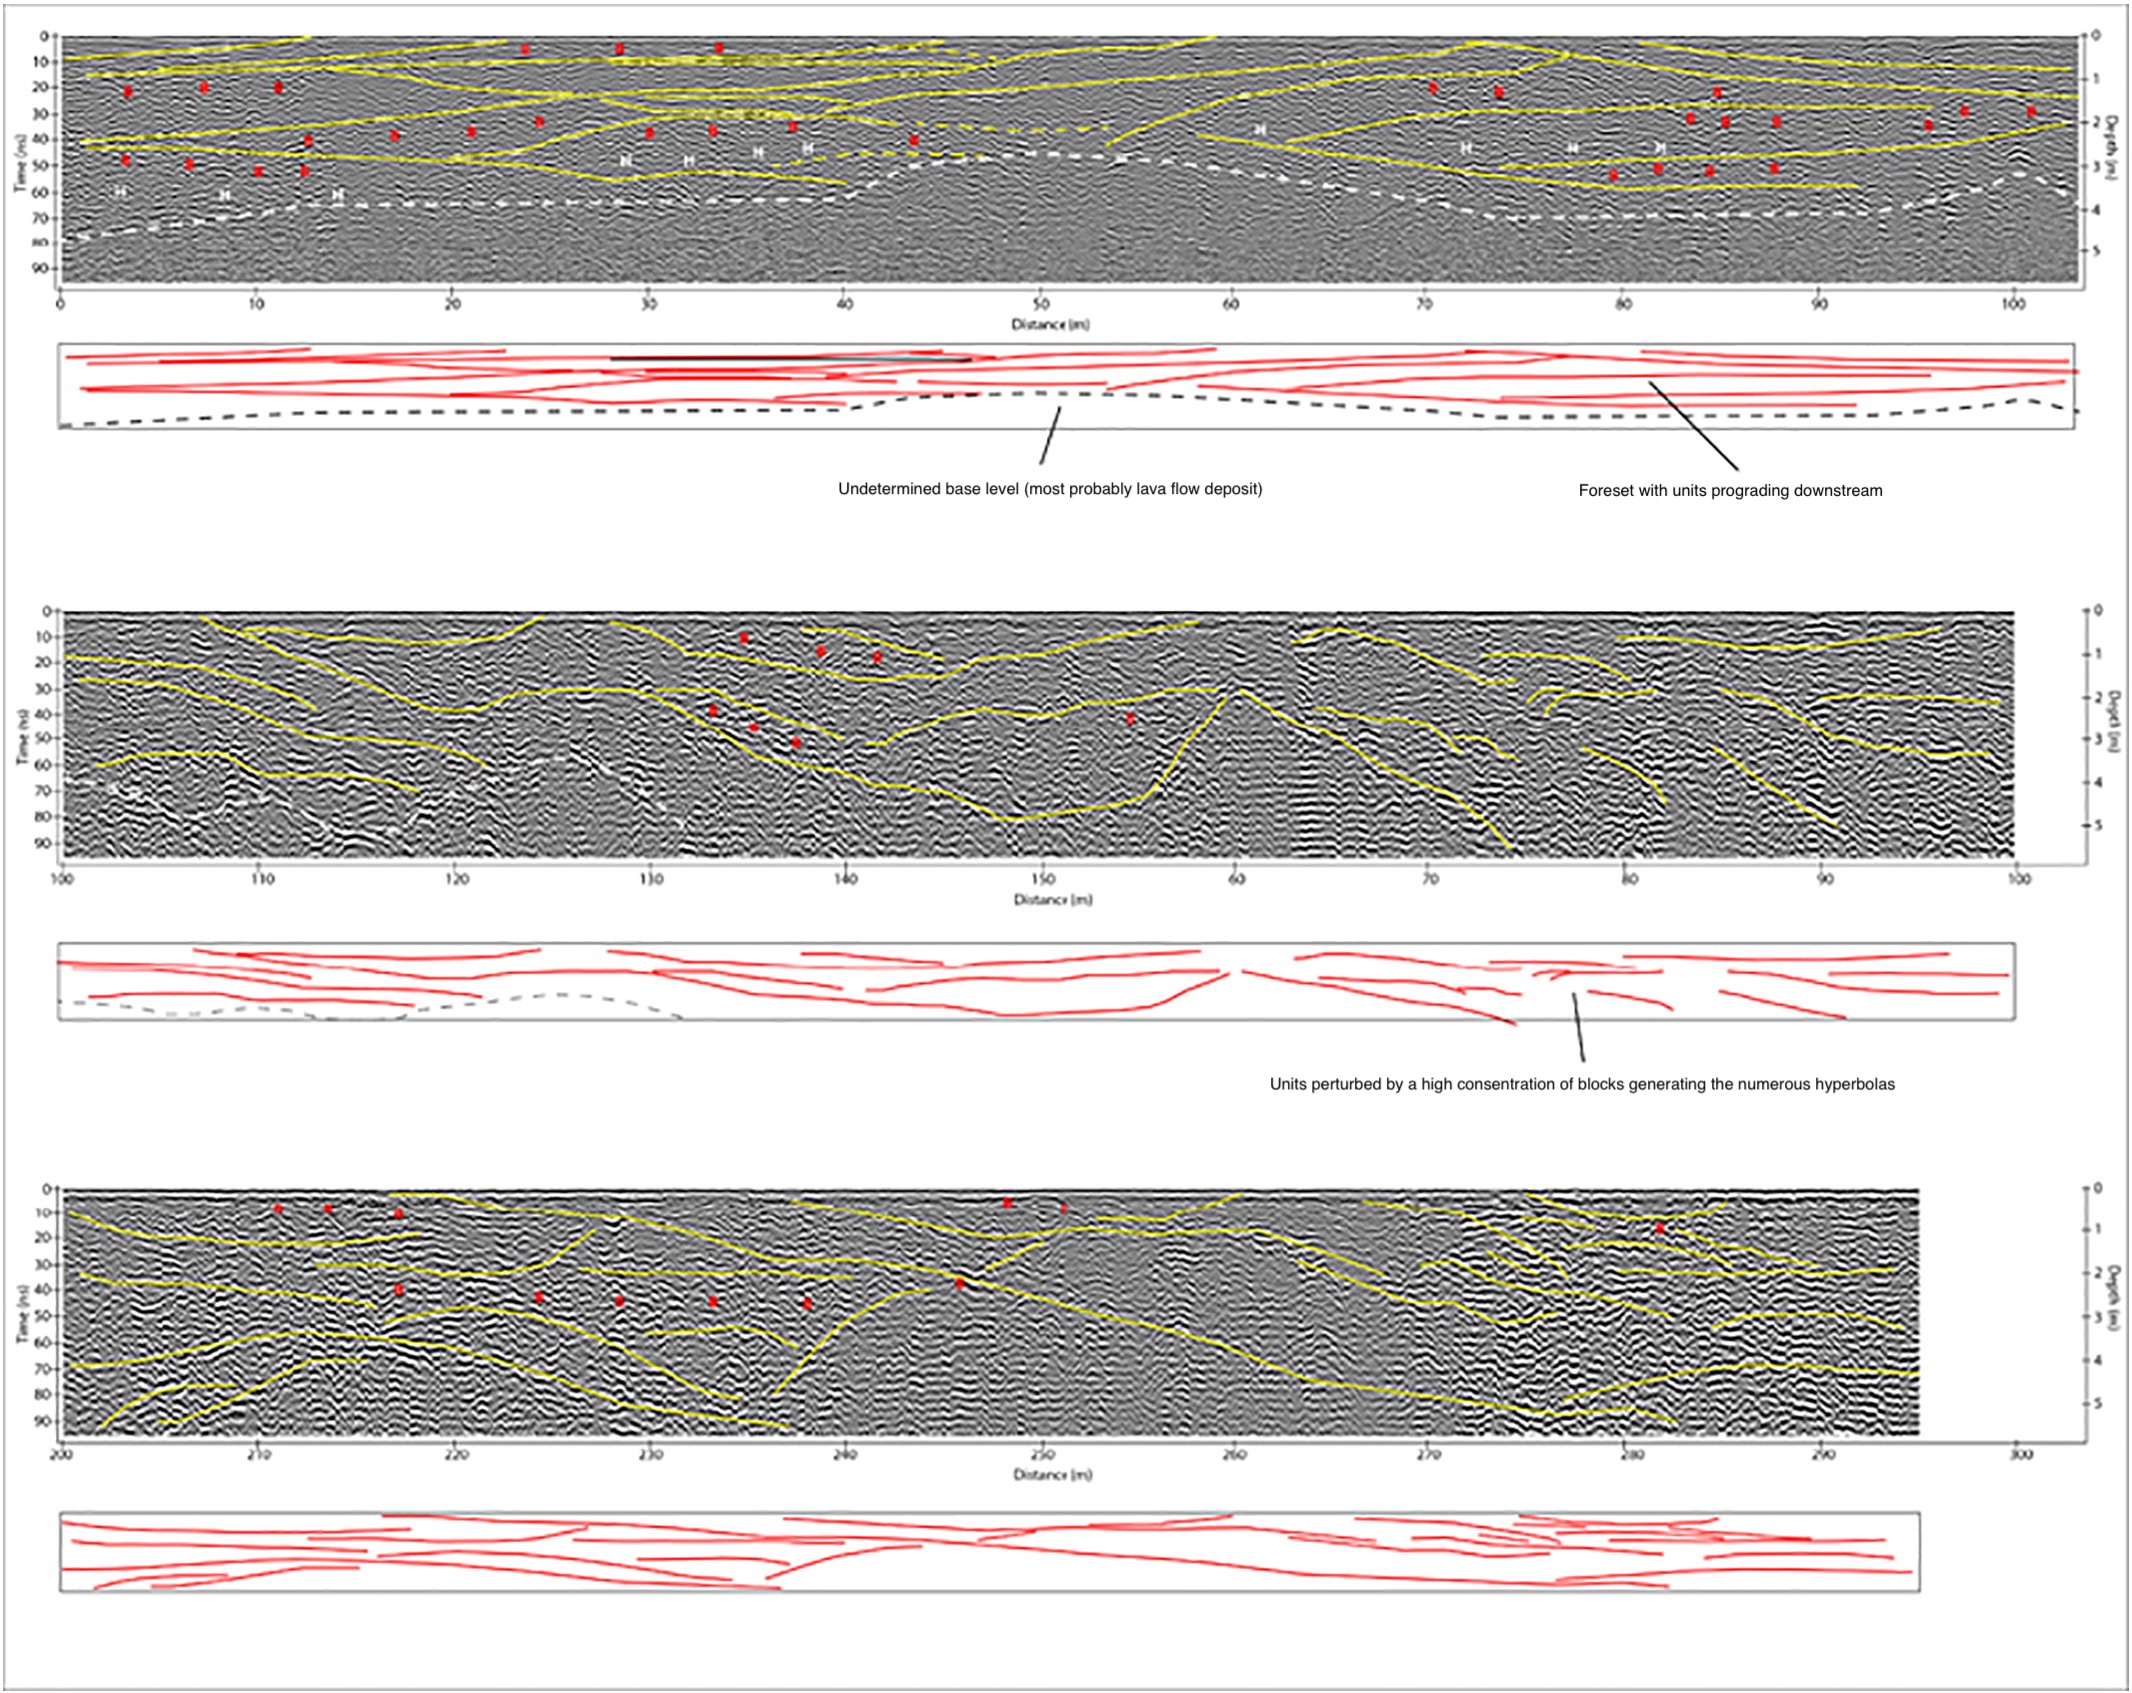
\includegraphics[width=0.9\linewidth]{Figures/0.2GPR/Gomez2018_1.jpg}
    \caption[Lahar deposit (1).]{Lahar deposit (1). \textbf{Keywords: } Concave up structures, prograding units, chaotic, truncation, hyperbolic, discontinuous, dipping, semi-continuous, multidirectional dipping, lenticular, low reflectivity.
   \citep{Gomez2018}.}
    \label{fig:Gomez2018-1}
\end{figure}

\begin{landscape}
    \begin{figure}[h!]
    \centering
    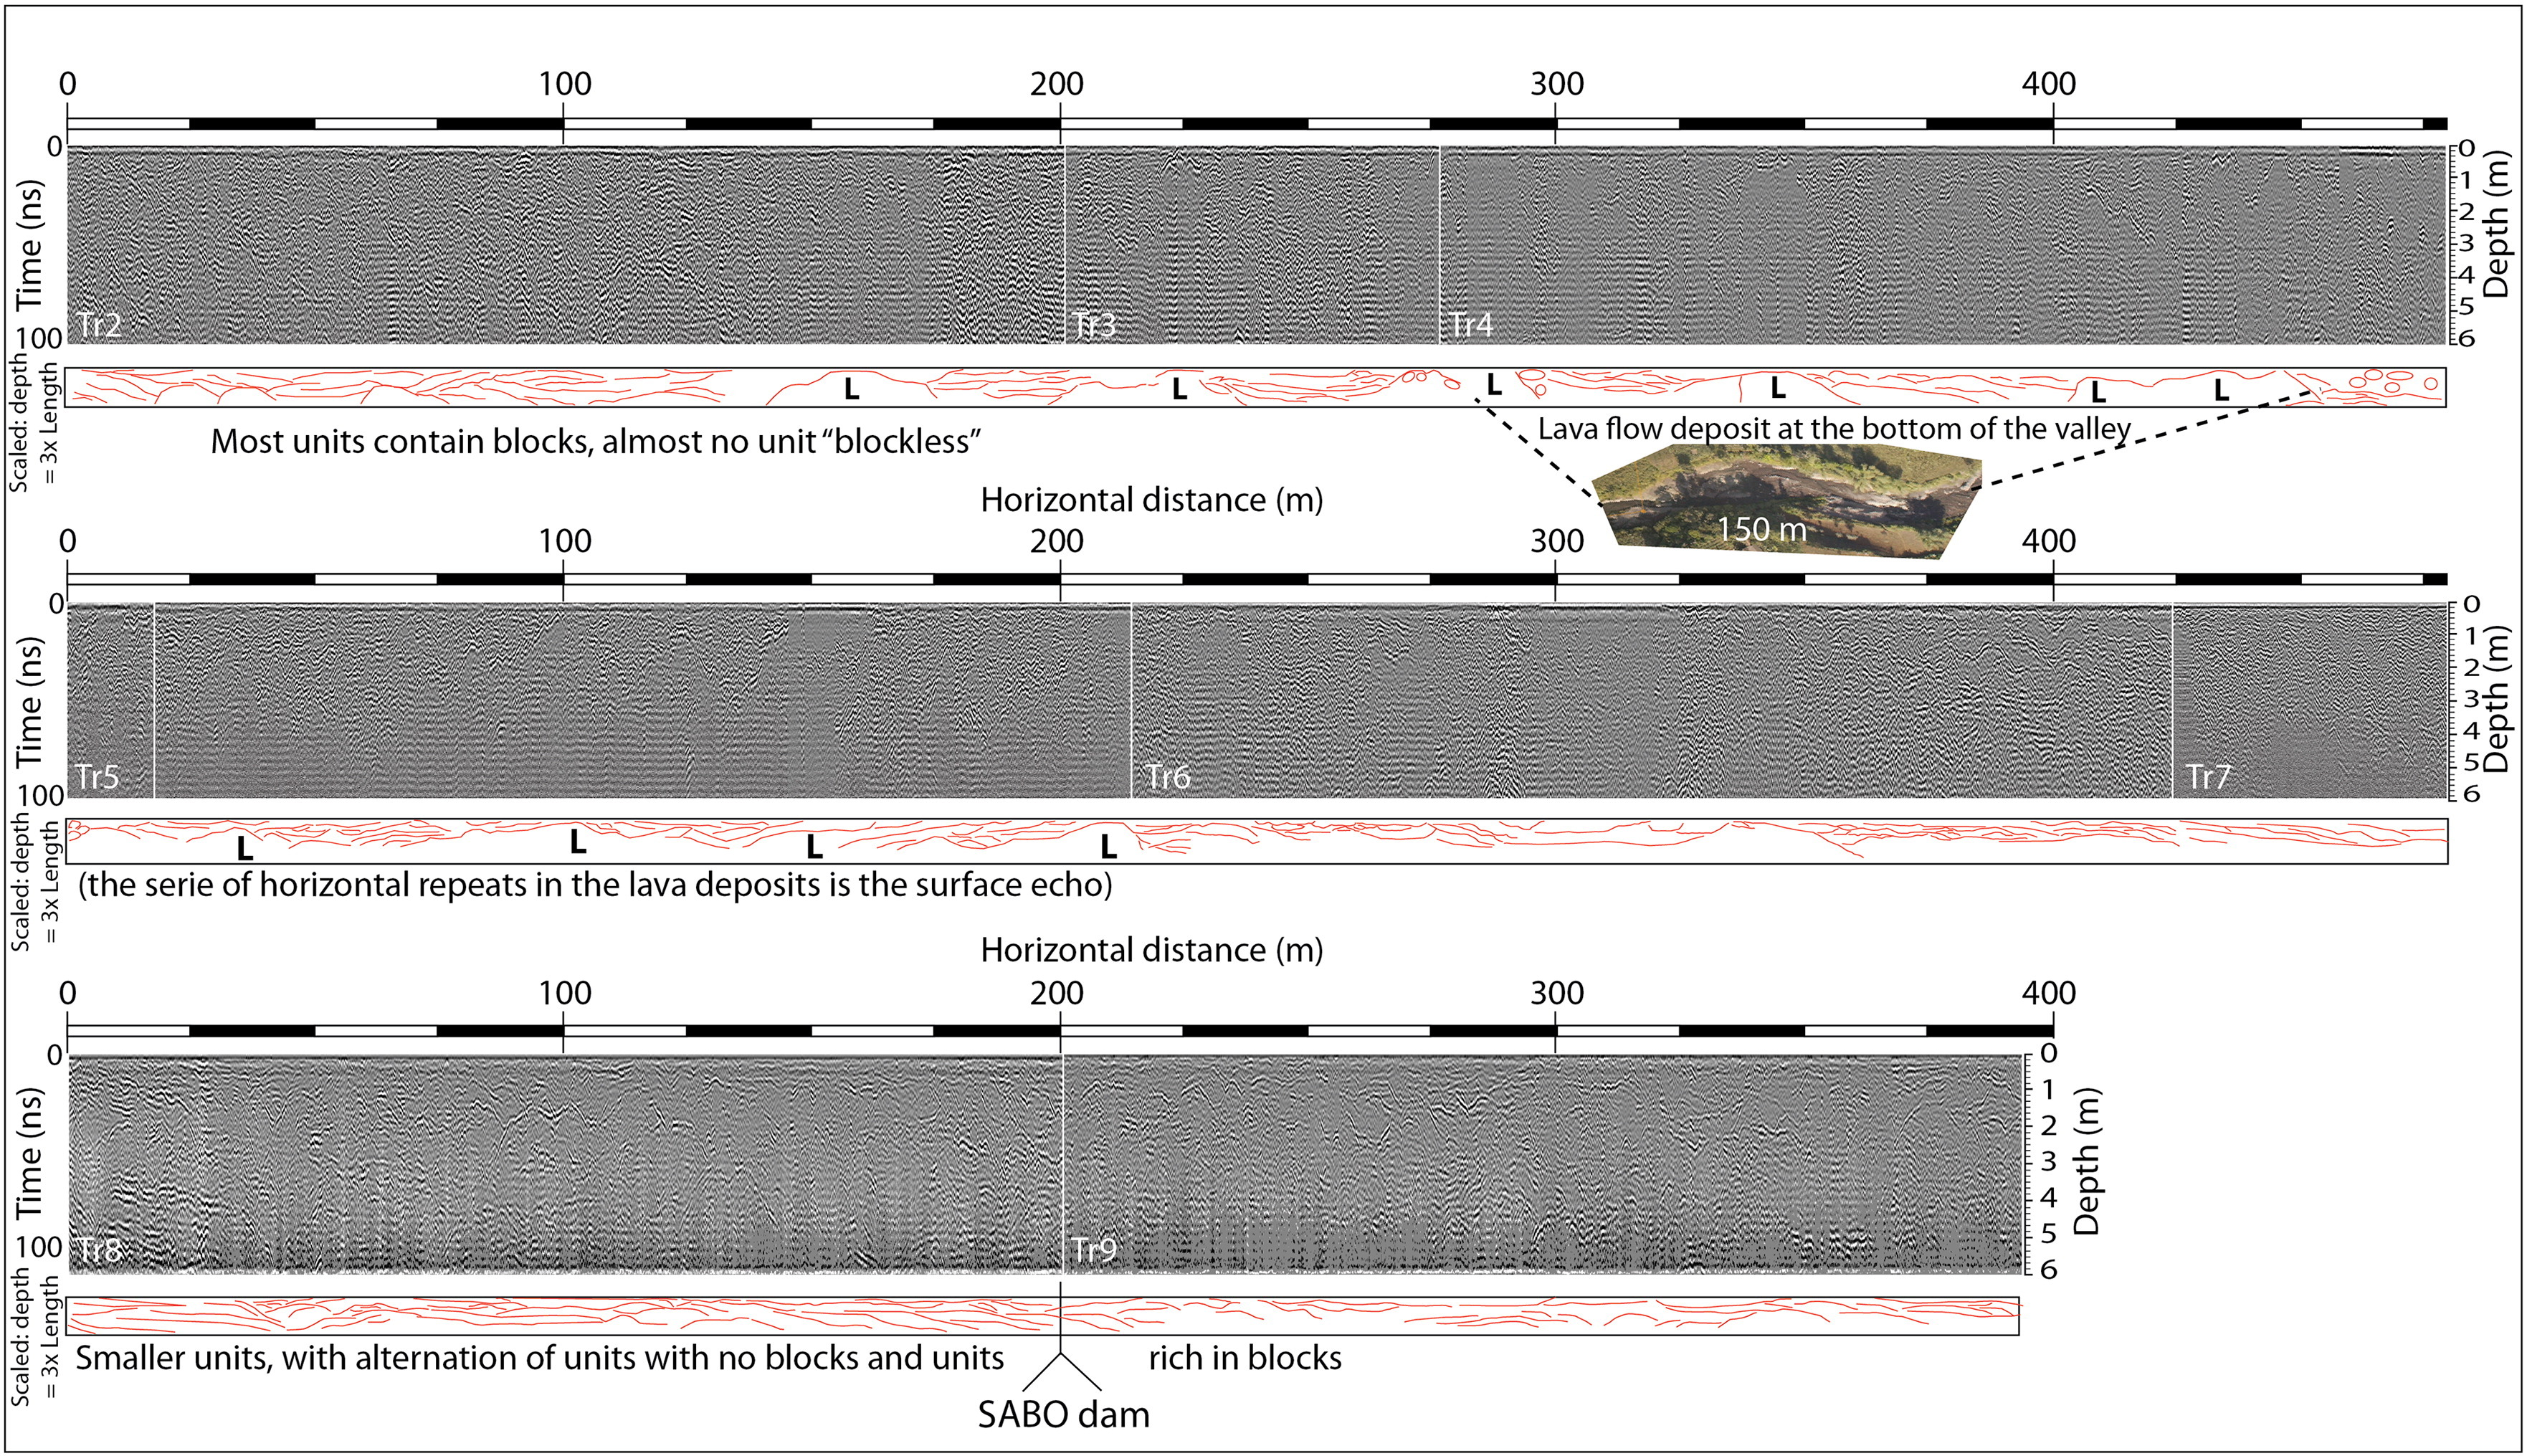
\includegraphics[width=0.9\linewidth]{Figures/0.2GPR/Gomez2018_2.jpg}
    \caption[Lahar deposit (2).]{Lahar deposit (2). \textbf{Keywords: } Horizontal layering, parallel, transparent zones, chaotic, discontinuous, alternating reflectivity, semi-continuous, dipping, high attenuation \citep{Gomez2018}.}
    \label{fig:Gomez2018-2}
\end{figure}
\end{landscape}
\clearpage

\begin{figure}[h!]
    \centering
    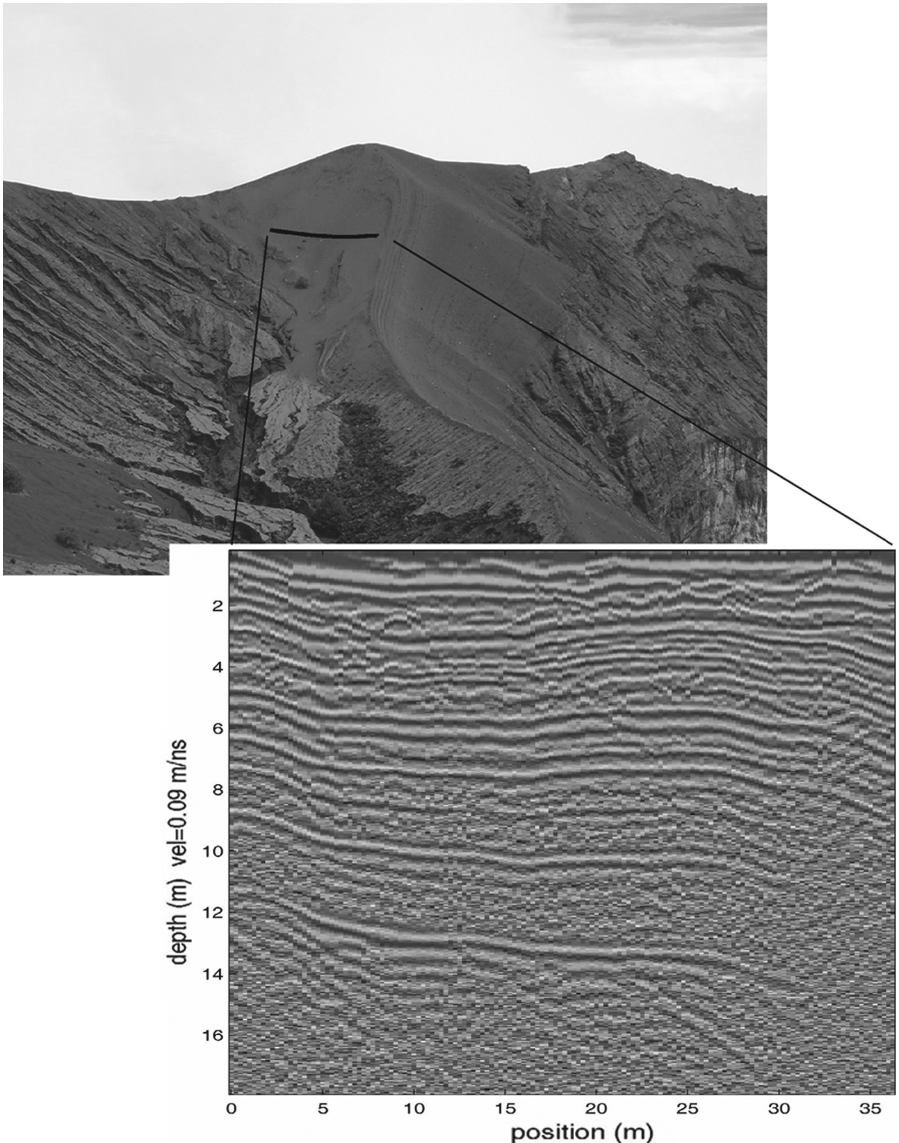
\includegraphics[width=0.9\linewidth]{Figures/0.2GPR/Kruse2010_tephra_3.png}
    \caption[Irazú intracrater tephra 1963-1965 deposits.]{\textbf{Keywords: } Parallel, semi-continous, dipping, hummocky, discontinous \citep{Kruse2010}.}
    \label{fig:Kruse2010-3}
\end{figure}
\clearpage

\begin{figure}[h!]
    \centering
    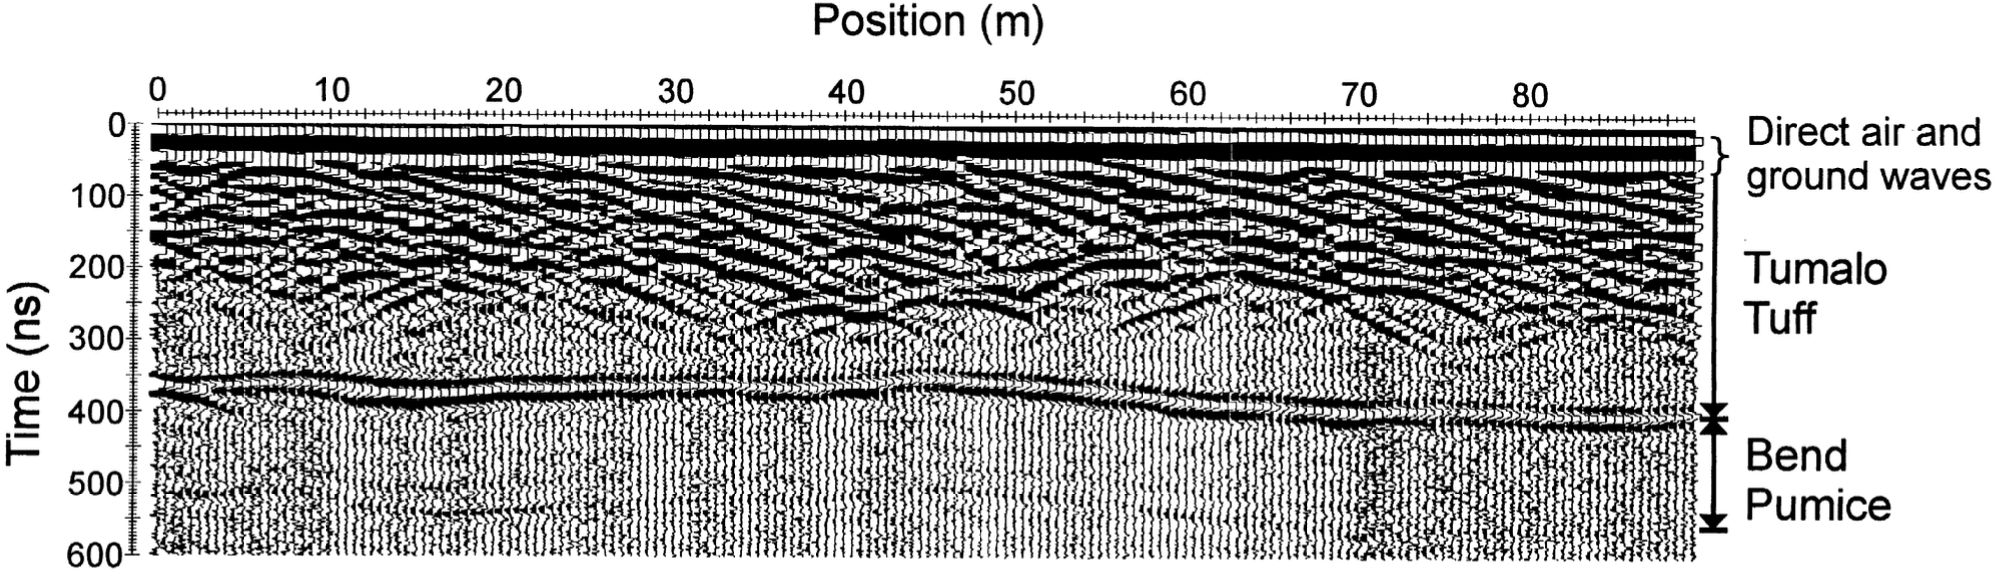
\includegraphics[width=0.9\linewidth]{Figures/0.2GPR/Rust2000_pyroclast_1.png}
    \caption[Welding in pyroclastic flows pre-migration.]{Welding in pyroclastic flows. \textbf{Keywords: } Parallel, dipping, sub-horizontal, continuous, discontinuous, varied attenuation, hummocky, crossing reflectors \citep{Rust2000}.}
    \label{fig:Rust2000-1}
\end{figure}

\begin{figure}[h!]
    \centering
    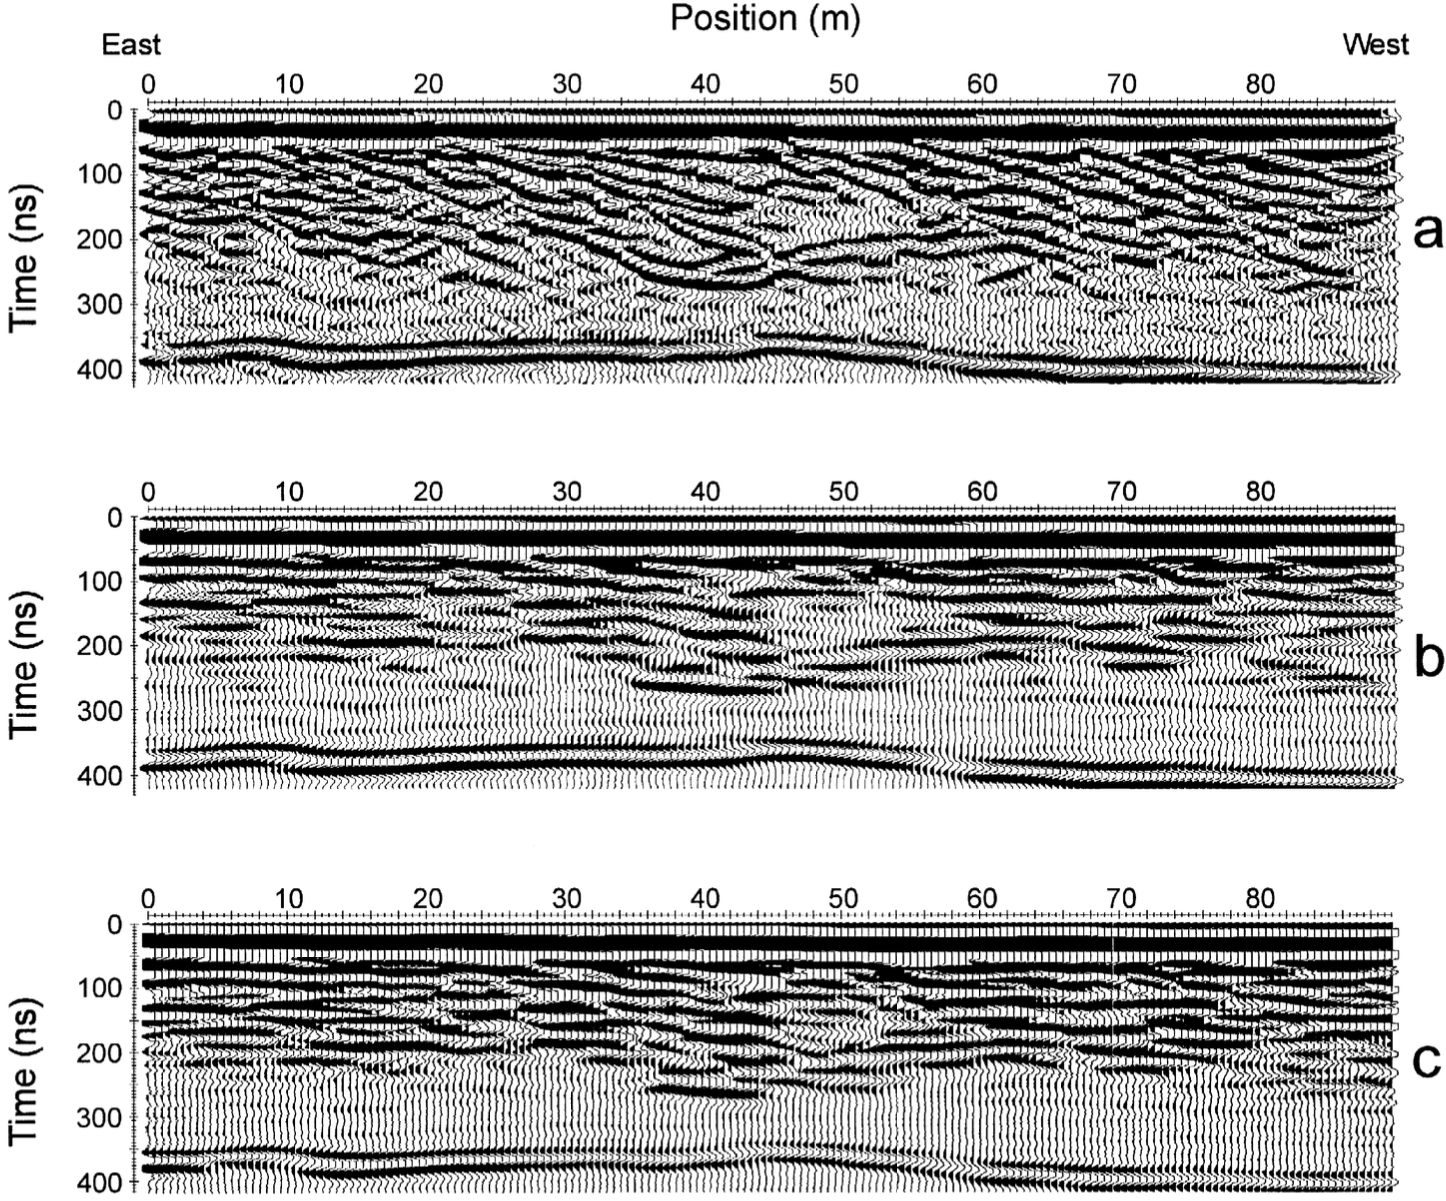
\includegraphics[width=0.9\linewidth]{Figures/0.2GPR/Rust2000_pyroclast_2.png}
    \caption[Welding in pyroclastic flows post-migration.]{Welding in pyroclastic flows. \textbf{Keywords: } Sub-horizontal, varied attenuation, semi-continuous, dipping, discontinuous, hummocky \citep{Rust2000}.}
    \label{fig:Rust2000-2}
\end{figure}
\clearpage


\begin{figure}[h!]
    \centering
    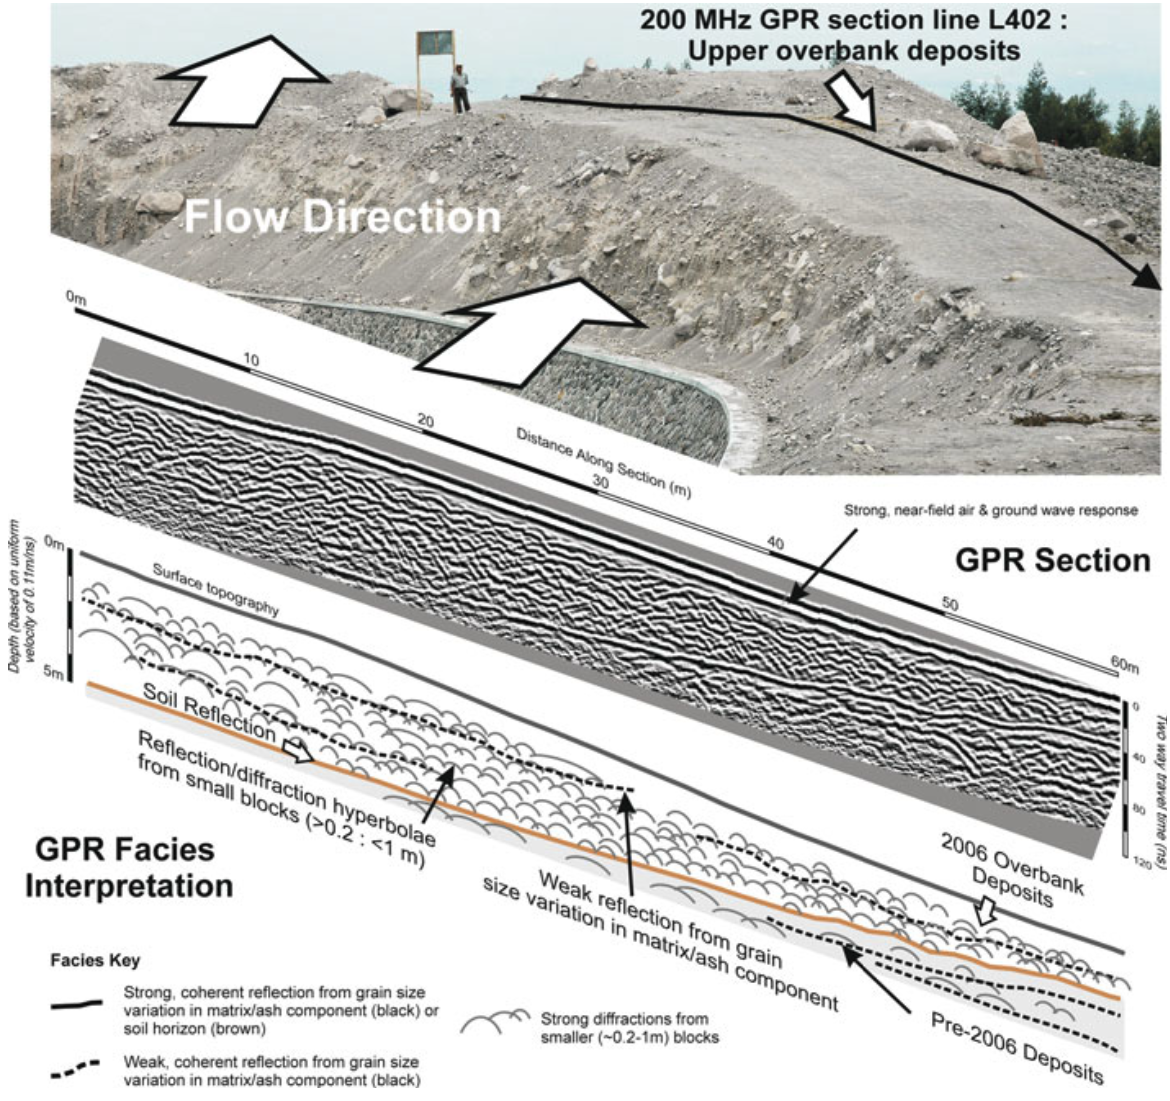
\includegraphics[width=0.9\linewidth]{Figures/0.2GPR/Gertisser2009_Block_Ash_1.png}
    \caption[Overbank block-and-ash flow deposits (1).]{Overbank block-and-ash flow deposits (1). \textbf{Keywords: } Differaction hyperbola, dipping, continuous, discontinuous, chaotic, low reflection \citep{Gertisser2012}.}
    \label{fig:Gertisser2012-1}
\end{figure}
\clearpage
\begin{figure}[h!]
    \centering
    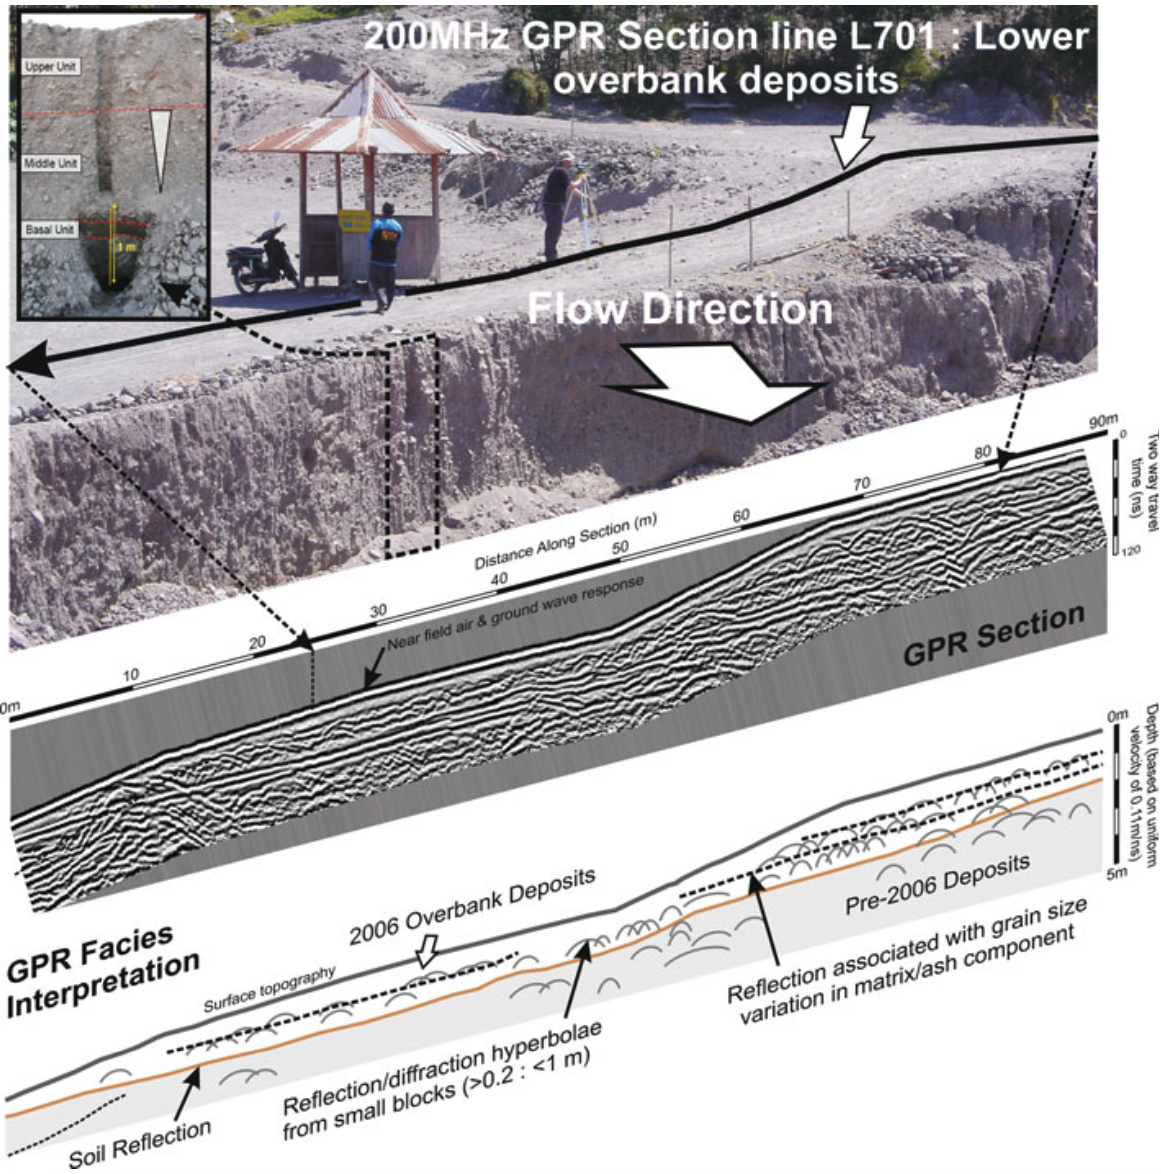
\includegraphics[width=0.9\linewidth]{Figures/0.2GPR/Gertisser2009_Block_Ash_2.png}
    \caption[Overbank block-and-ash flow deposits (2).]{Overbank block-and-ash flow deposits (2). \textbf{Keywords: } Differaction hyperbola, dipping, horizontal, semi-continuous, discontinuous, high reflectivity, continuous \citep{Gertisser2012}.}
    \label{fig:Gertisser2012-2}
\end{figure}
\clearpage

\begin{figure}[h!]
    \centering
    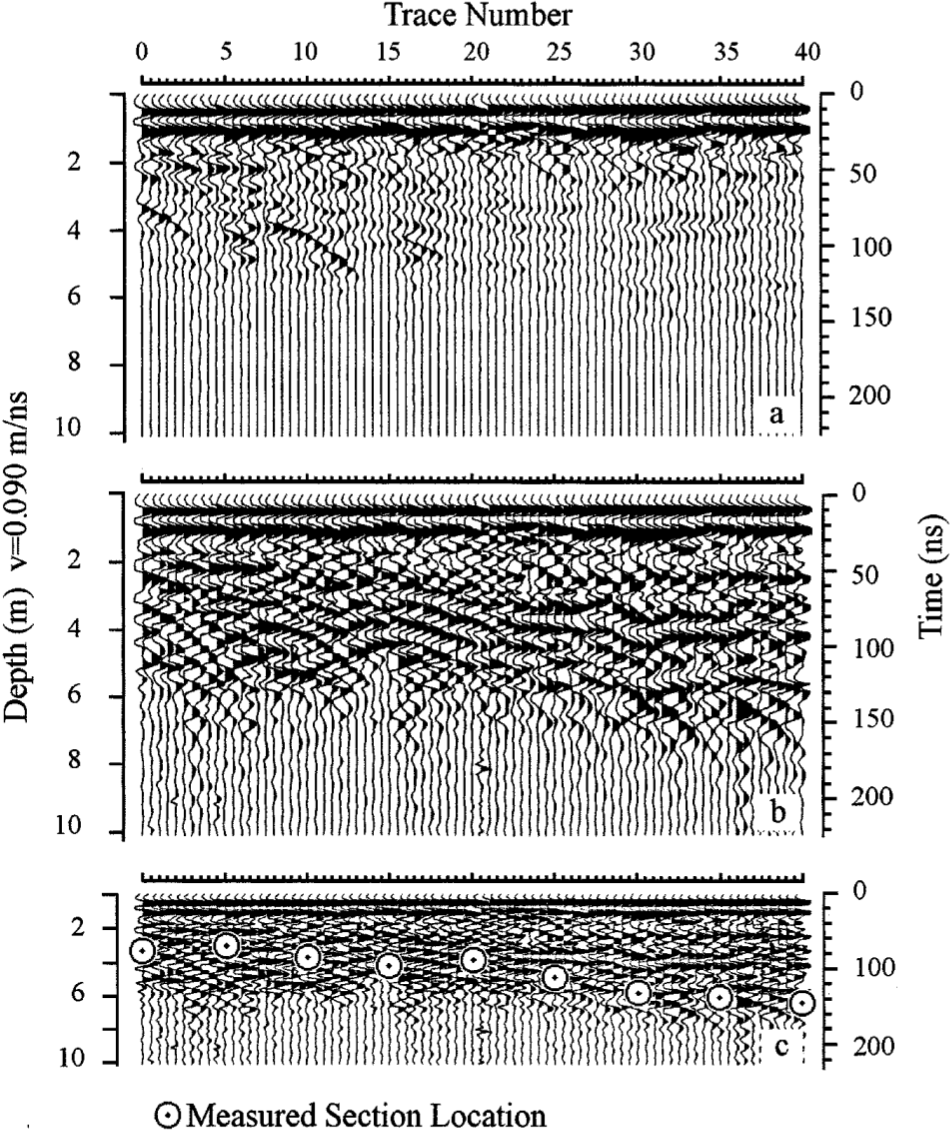
\includegraphics[width=0.9\linewidth]{Figures/0.2GPR/Russel1996_volcanic_deposits_1.png}
    \caption[Basalt lava flow (1).]{Basalt lava flow (1). \textbf{Keyword:} Hummocky, irregular, discontinuous, dipping, high attenuation, horizontal, crossing reflectors \citep{Russell1997}.}
    \label{fig:Russell1996-1}
\end{figure}

\begin{figure}[h!]
    \centering
    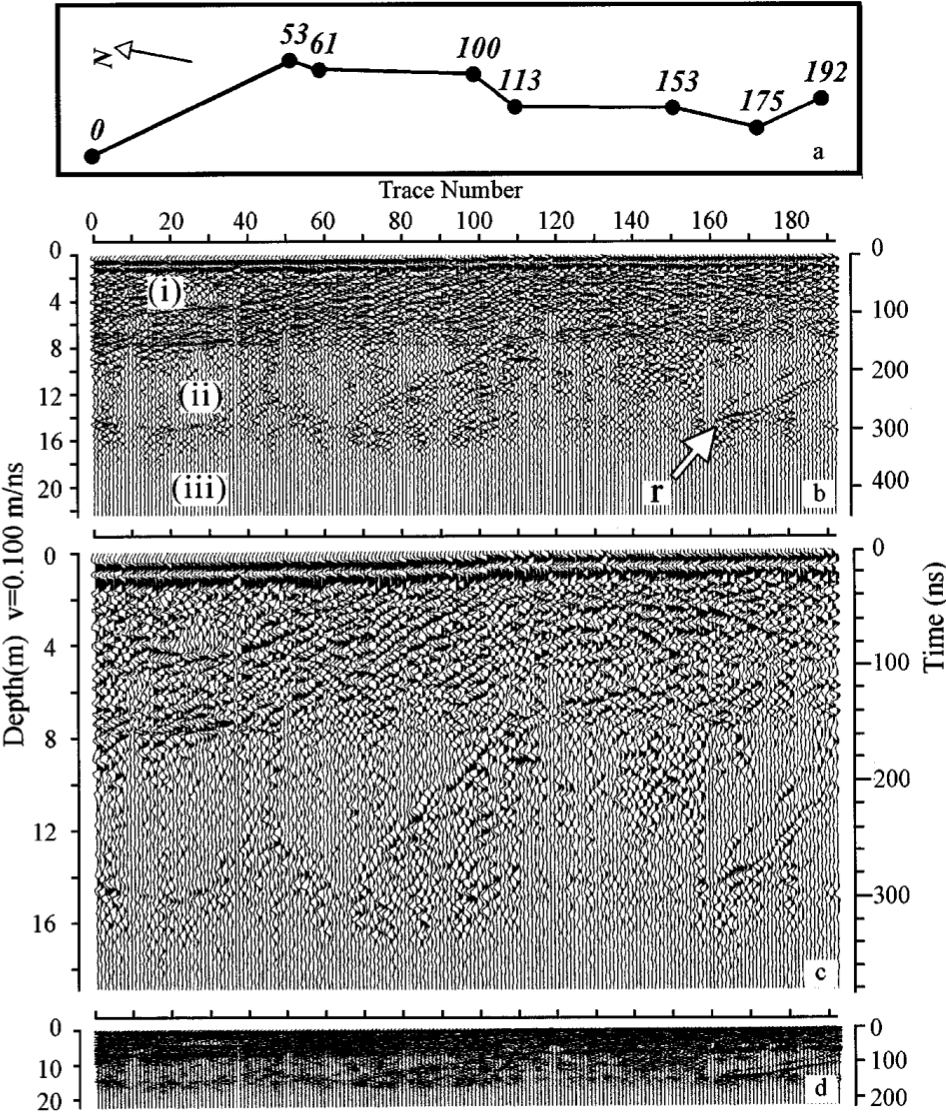
\includegraphics[width=0.9\linewidth]{Figures/0.2GPR/Russel1996_volcanic_deposits_3.png}
    \caption[Basalt lava flow (2).]{Basalt lava flow (1). \textbf{Keywords: } Dipping, high attenuation, discontinuous, horizontal, multidirectional dipping \citep{Russell1997}.}
    \label{fig:Russel2017-3}
\end{figure}

\begin{landscape}
\begin{figure}[h!]
    \centering
    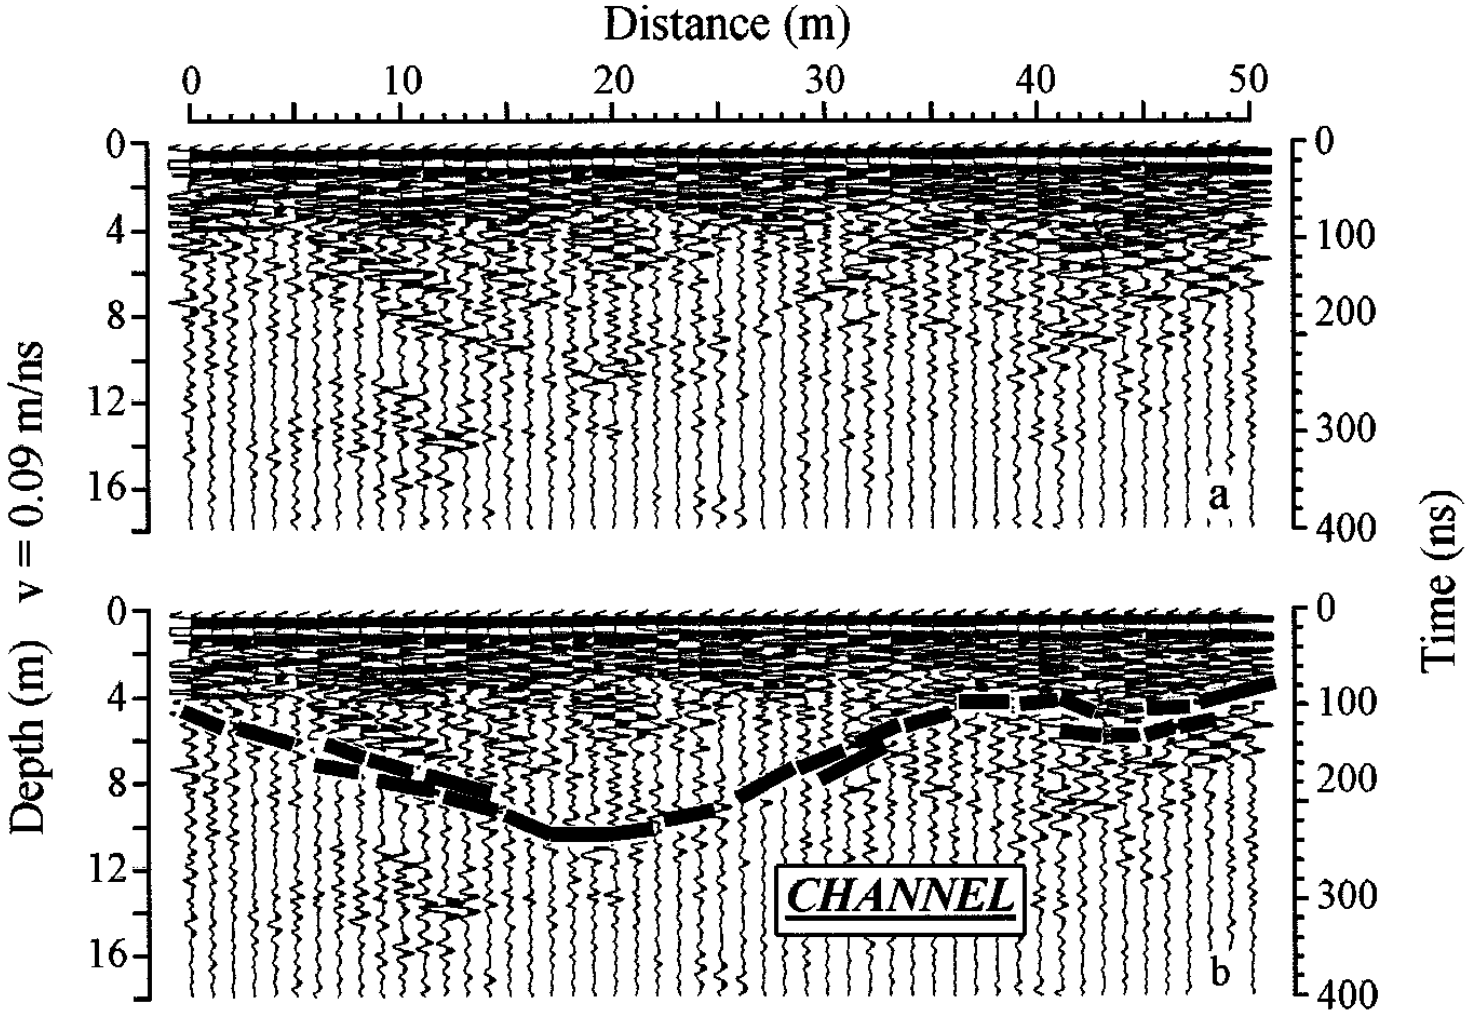
\includegraphics[width=0.9\linewidth]{Figures/0.2GPR/Russel1996_volcanic_deposits_5.png}
    \caption[Pumice talus deposit.]{Pumice talus deposit. \textbf{Keywords: } Discontinuous, dipping, high attenuation, horizontal, multidirectional dipping, hummocky, concave \citep{Russell1997}.}
    \label{fig:Russell1996-5}
\end{figure}
\end{landscape}
\clearpage